La siguiente figura representa el flujo de autos según el horario del día:
\begin{figure}[ht!]
    \centering
    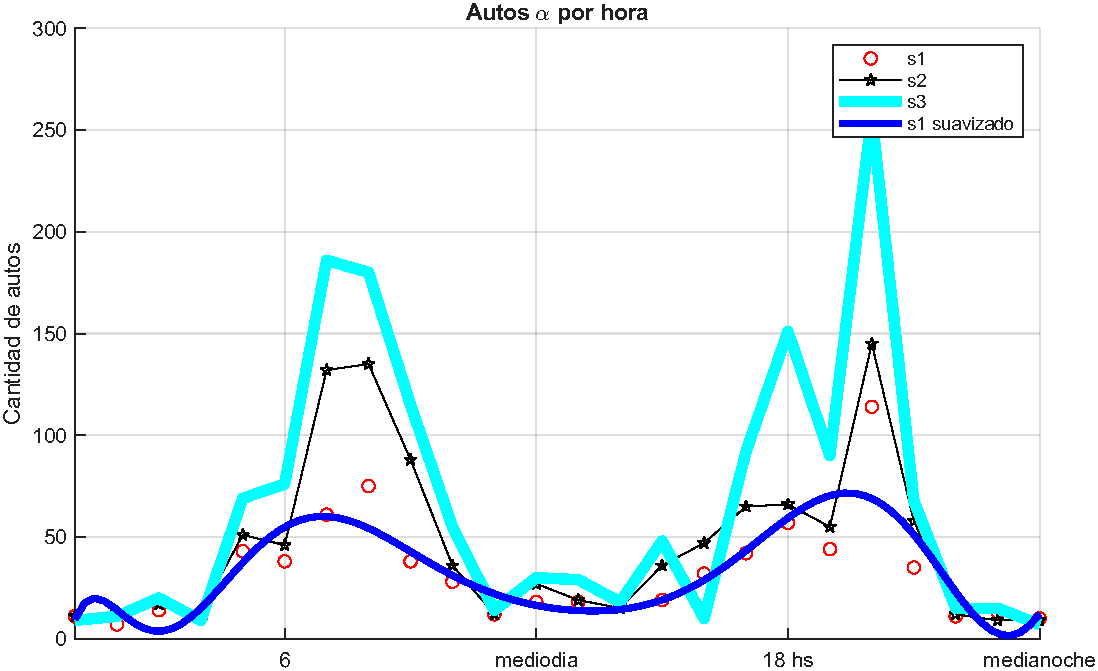
\includegraphics[width=0.8\textwidth]{imagenes/auto_por_dia.pdf}
    \caption{Flujo de autos por horarios}
    \label{fig:1}
\end{figure}



Se observa del gráfico que la gente de Natick trabaja de 8 am hasta las 5 pm, donde el flujo de autos es menor. El siguiente código muestra cómo se hizo el gráfico:

\begin{lstlisting}
clear all;
load count.dat;


fig = figure('Name', 'Guia 03', 'PaperPosition', [0, 0, 30, 15]);
theme(fig, 'light');
grid on;
hold on;

t = 1:24;
tsuave = linspace(1, 24, 100);

%3 señales
s1 = count(:, 1);
s2 = count(:, 2);
s3 = count(:, 3);


%Interpolacion
coef1 = polyfit(t, s1, 10);
s1_suave = polyval(coef1, tsuave);    

%ploteo
plot(t, s1, 'ro')
plot(t, s2, 'pentagram-', Color='black')
plot(t, s3, Color='cyan', LineWidth=5)
plot(tsuave, s1_suave, Color='blue', LineWidth=3)
title('Autos \alpha por hora')
ylabel('Cantidad de autos')
legend('s1', 's2', 's3', 's1 suavizado')
set(gca,'XLimMode','manual','XLim',[1 24]);
set(gca,'XTick',6:6:24); % etiquetas a las horas: 6,12,18 y 24.
set(gca,'XTickLabel',{'6';'mediodia';'18 hs';'medianoche'});
set(gca,'XGrid','on')
\end{lstlisting}


El siguiente gráfico representa un gráfico 3D:

\begin{figure}[ht!]
    \centering
    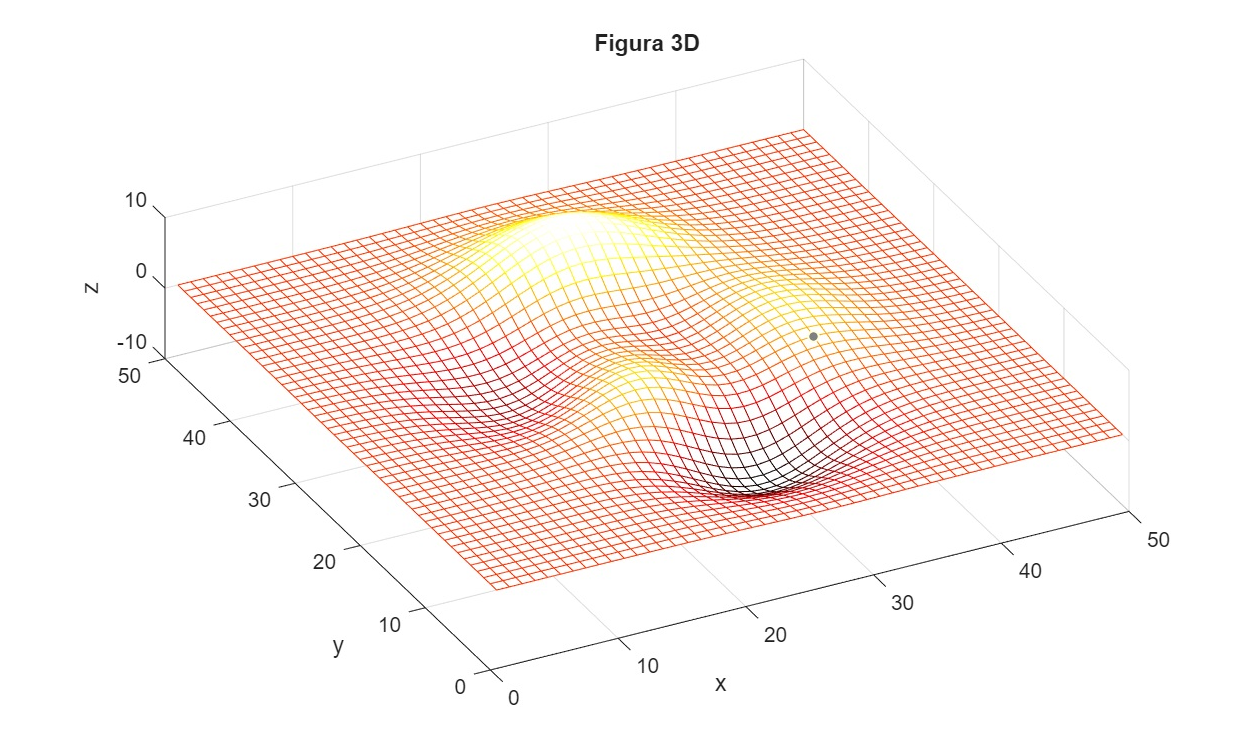
\includegraphics[width=0.8\textwidth]{imagenes/3d_plot.pdf}
    \caption{Gráfico 3D en MATLAB}
    \label{fig:2}
\end{figure}


\noindent El código es:

\begin{lstlisting}
fig2 = figure;
theme(fig2, 'light')
z = peaks(50); %Si aumento el numero densifico mas la malla
mesh(z)
colormap("hot")
xlabel('x')
ylabel('y')
zlabel('z')
title('Figura 3D')
view([-27, 68]) %Con esto modifico la vista inicial
\end{lstlisting}
